
\documentclass[sigconf]{acmart}

\AtBeginDocument{%
  \providecommand\BibTeX{{%
    \normalfont B\kern-0.5em{\scshape i\kern-0.25em b}\kern-0.8em\TeX}}}

\copyrightyear{2021}
\acmYear{2021}
\setcopyright{acmlicensed}
\acmConference[Web3D '21]{The 26th International Conference on 3D Web Technology}{November 8--12, 2021}{Pisa, Italy}
\acmBooktitle{The 26th International Conference on 3D Web Technology (Web3D '21), November 8--12, 2021, Pisa, Italy}
\acmPrice{15.00}
\acmDOI{10.1145/3485444.3487640}
\acmISBN{978-1-4503-9095-8/21/11}

\acmSubmissionID{2}

\citestyle{acmauthoryear}

\usepackage[nameinlink,noabbrev]{cleveref}
\crefname{lstlisting}{listing}{listings}
\Crefname{lstlisting}{Listing}{Listings}

\usepackage{siunitx}
\usepackage{tabularx}
\usepackage{xcolor}

\usepackage{tikz}
\usetikzlibrary{calc,positioning,spy,shapes}

\usepackage{listings} 
\usepackage{accsupp}

% from Daniel Limbergers custom PhD Thesis Styles

\lstset{
    basicstyle        = \ttfamily\lst@ifdisplaystyle\scriptsize\fi %
,   sensitive         = true
,   columns           = flexible
,   keepspaces        = true
,   emptylines        = 2
,   upquote           = true
,   tabsize           = 4
,   numbers           = left
,   numbersep         = 3.0em
,   numberstyle       = \ttfamily\tiny\color{lightgray}
,   numberblanklines  = false
,   resetmargins      = true
,   xleftmargin       = 3.0em
,   frame             = leftline
,   framesep          = 1.5em
,   rulecolor         = \color{darkgray}
,	literate          = *
,   keywordstyle      = \lst@ifdisplaystyle\bfseries\color{black}\fi
,   identifierstyle   = \lst@ifdisplaystyle\color{black}\fi
,   commentstyle      = \lst@ifdisplaystyle\color{lightgray}\fi
,   stringstyle       = \color{darkgray}
,   showstringspaces  = false
,   captionpos        = b
}

% from Daniel Limbergers custom PhD Thesis Styles

\lstdefinelanguage{glsl}
{
    style             = glsl
,   morekeywords      = [1]{%
        attribute,const,uniform,varying,layout,centroid,flat,smooth,noperspective,break,continue,do,for,while,switch,case,default,if,else,in,out,inout,float,int,void,bool,true,false,invariant,discard,return,mat2,mat3,mat4,mat2x2,mat2x3,mat2x4,mat3x2,mat3x3,mat3x4,mat4x2,mat4x3,mat4x4,vec2,vec3,vec4,ivec2,ivec3,ivec4,bvec2,bvec3,bvec4,uint,uvec2,uvec3,uvec4,lowp,mediump,highp,precision,sampler1D,sampler2D,sampler3D,samplerCube,sampler1DShadow,sampler2DShadow,samplerCubeShadow,sampler1DArray,sampler2DArray,sampler1DArrayShadow,sampler2DArrayShadow,isampler1D,isampler2D,isampler3D,isamplerCube,isampler1DArray,isampler2DArray,usampler1D,usampler2D,usampler3D,usamplerCube,usampler1DArray,usampler2DArray,sampler2DRect,sampler2DRectShadow,isampler2DRect,usampler2DRect,samplerBuffer,isamplerBuffer,usamplerBuffer,sampler2DMS,isampler2DMS,usampler2DMS,sampler2DMSArray,isampler2DMSArray,usampler2DMSArray,struct}
,	morekeywords      = [2]{%
    radians,degrees,sin,cos,tan,asin,acos,atan,atan,sinh,cosh,tanh,asinh,acosh,atanh,pow,exp,log,exp2,log2,sqrt,inversesqrt,abs,sign,floor,trunc,round,roundEven,ceil,fract,mod,modf,min,max,clamp,mix,step,smoothstep,isnan,isinf,floatBitsToInt,floatBitsToUint,intBitsToFloat,uintBitsToFloat,length,distance,dot,cross,normalize,faceforward,reflect,refract,matrixCompMult,outerProduct,transpose,determinant,inverse,lessThan,lessThanEqual,greaterThan,greaterThanEqual,equal,notEqual,any,all,not,textureSize,texture,textureProj,textureLod,textureOffset,texelFetch,texelFetchOffset,textureProjOffset,textureLodOffset,textureProjLod,textureProjLodOffset,textureGrad,textureGradOffset,textureProjGrad,textureProjGradOffset,texture1D,texture1DProj,texture1DProjLod,texture2D,texture2DProj,texture2DLod,texture2DProjLod,texture3D,texture3DProj,texture3DLod,texture3DProjLod,textureCube,textureCubeLod,shadow1D,shadow2D,shadow1DProj,shadow2DProj,shadow1DLod,shadow2DLod,shadow1DProjLod,shadow2DProjLod,dFdx,dFdy,fwidth,noise1,noise2,noise3,noise4,EmitVertex,EndPrimitive}
,	morekeywords      = [3]{%
        gl_VertexID,gl_InstanceID,gl_Position,gl_PointSize,gl_ClipDistance,gl_PerVertex,gl_Layer,gl_ClipVertex,gl_FragCoord,gl_FrontFacing,gl_ClipDistance,gl_FragColor,gl_FragData,gl_MaxDrawBuffers,gl_FragDepth,gl_PointCoord,gl_PrimitiveID,gl_MaxVertexAttribs,gl_MaxVertexUniformComponents,gl_MaxVaryingFloats,gl_MaxVaryingComponents,gl_MaxVertexOutputComponents,gl_MaxGeometryInputComponents,gl_MaxGeometryOutputComponents,gl_MaxFragmentInputComponents,gl_MaxVertexTextureImageUnits,gl_MaxCombinedTextureImageUnits,gl_MaxTextureImageUnits,gl_MaxFragmentUniformComponents,gl_MaxDrawBuffers,gl_MaxClipDistances,gl_MaxGeometryTextureImageUnits,gl_MaxGeometryOutputVertices,gl_MaxGeometryOutputVertices,gl_MaxGeometryTotalOutputComponents,gl_MaxGeometryUniformComponents,gl_MaxGeometryVaryingComponents,gl_DepthRange}
,   morestring        = [b]'
,   morestring        = [b]"
,	morecomment       = [l]{//}
,	morecomment       = [s]{/*}{*/}
,	morecomment       = [l][keywordstyle4]{\#}
}

\lstdefinestyle{glsl}
{
}

\lstset{inputpath={listings/}}

\usepackage{csquotes}


\begin{document}

\title{Interactive Volumetric Region Growing for Brain Tumor Segmentation on MRI using WebGL}

\author{Jonas Kordt}
\affiliation{%
  \institution{Hasso Plattner Institute - University of Potsdam}
  \city{Potsdam}
  \country{Germany}
  \postcode{14482}
}
\email{jonas.kordt@student.hpi.de}

\author{Paul Brachmann}
\affiliation{%
  \institution{Hasso Plattner Institute - University of Potsdam}
  \city{Potsdam}
  \country{Germany}
  \postcode{14482}
}
\email{paul.brachmann@hpi.de}

\author{Daniel Limberger}
\affiliation{%
  \institution{Hasso Plattner Institute - University of Potsdam}
  \city{Potsdam}
  \country{Germany}
  \postcode{14482}
}
\email{daniel.limberger@hpi.de}

\author{Christoph Lippert}
\affiliation{%
  \institution{Hasso Plattner Institute - University of Potsdam}
  \city{Potsdam}
  \country{Germany}
  \postcode{14482}
}
\email{christoph.lippert@hpi.de}

\begin{abstract}
Volumetric segmentation of medical images is an essential tool in treatment planning and many longitudinal studies. While machine learning approaches promise to fully automate it, they most often still depend on manually labeled training data. We thus present a GPU-based volumetric region growing approach for semi-automatic brain tumor segmentation that can be interactively tuned. Additionally, we propose multidimensional transfer functions for ray tracing that allow users to judge the quality of the grown region. Our implementation produces a full brain tumor segmentation within a few milliseconds on consumer hardware. The visualization uses adaptive resolution scaling and progressive, asynchronous shading computation to maintain a stable $60$ Hz refresh rate.
\end{abstract}

\begin{CCSXML}
<ccs2012>
   <concept>
       <concept_id>10010147.10010371</concept_id>
       <concept_desc>Computing methodologies~Computer graphics</concept_desc>
       <concept_significance>300</concept_significance>
       </concept>
   <concept>
       <concept_id>10003120.10003145</concept_id>
       <concept_desc>Human-centered computing~Visualization</concept_desc>
       <concept_significance>500</concept_significance>
       </concept>
   <concept>
       <concept_id>10003120.10003121</concept_id>
       <concept_desc>Human-centered computing~Human computer interaction (HCI)</concept_desc>
       <concept_significance>300</concept_significance>
       </concept>
   <concept>
       <concept_id>10010405.10010444</concept_id>
       <concept_desc>Applied computing~Life and medical sciences</concept_desc>
       <concept_significance>100</concept_significance>
       </concept>
 </ccs2012>
\end{CCSXML}

\ccsdesc[500]{Human-centered computing~Visualization}
\ccsdesc[300]{Human-centered computing~Human computer interaction (HCI)}
\ccsdesc[300]{Applied computing~Life and medical sciences}
\ccsdesc[100]{Computing methodologies~Computer graphics}

\keywords{medical imaging, MRI, brain tumor, interactive segmentation, data labeling, region growing, progressive rendering, WebGL}

\begin{teaserfigure}
    \begin{tikzpicture}[%
        every node/.append style={shape=rectangle, rounded corners=2mm}, %
        spy using outlines={white, rectangle, magnification=2.0, size=64, connect spies, every spy on node/.append style={line width=1.0pt}}, %
        inner sep=0pt, outer sep=0pt]
        \node[anchor=west, clip](scans) at (0,0) {%
            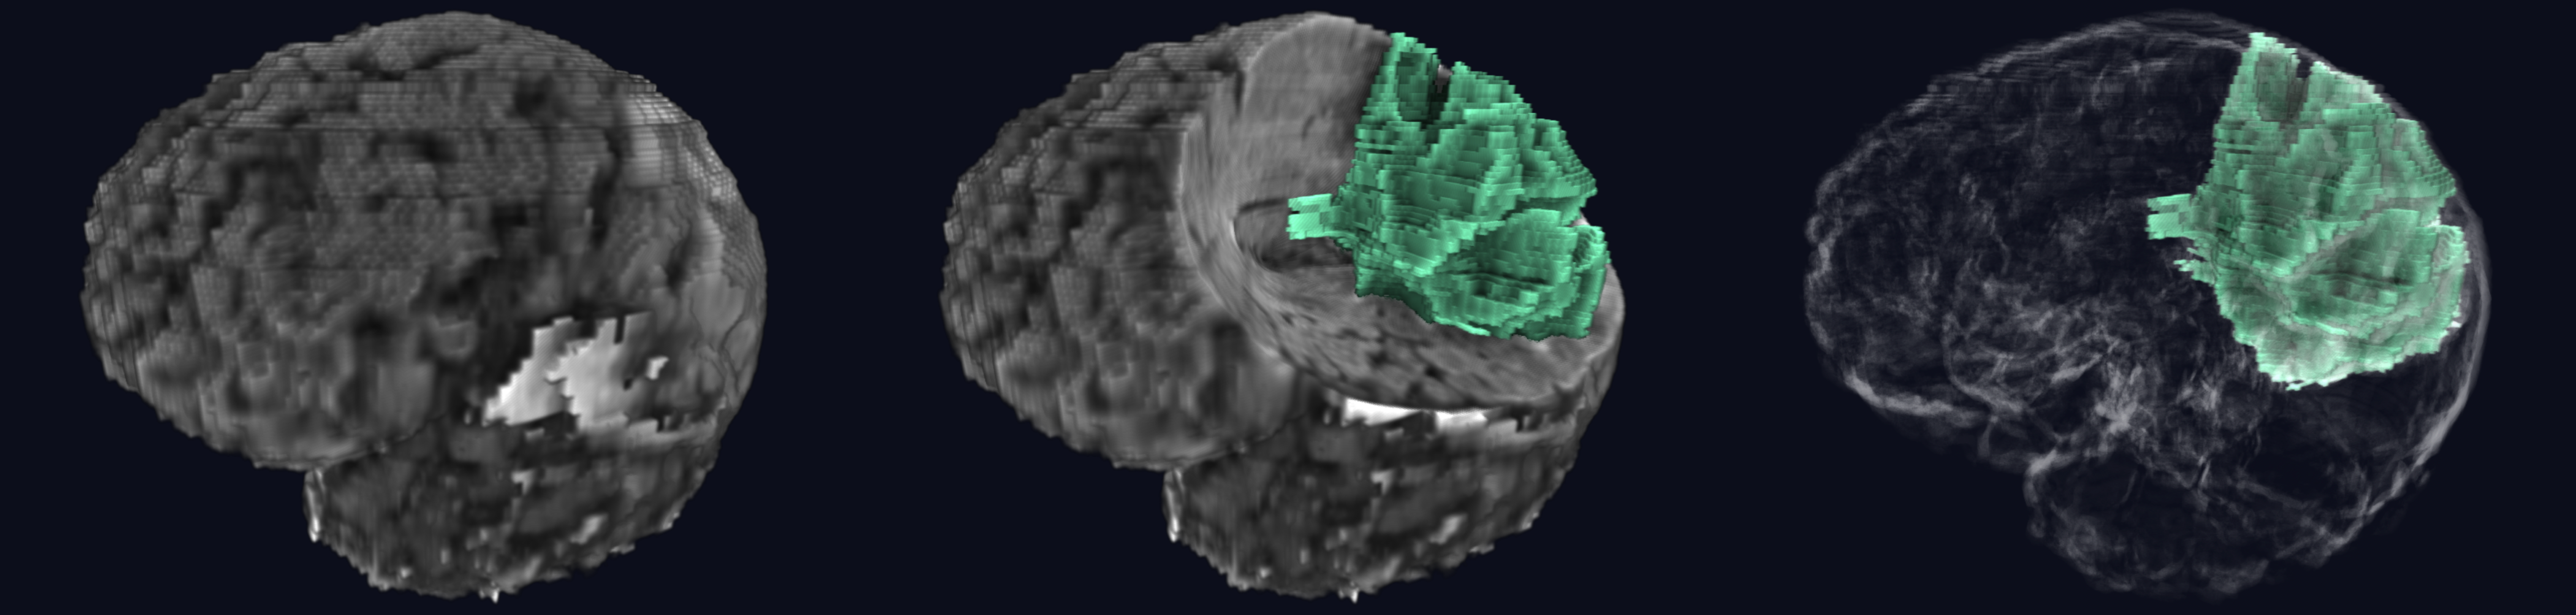
\includegraphics[width=1.0\linewidth, trim=0 0 0 0, clip]{figures/teaser}};
    \end{tikzpicture}
    \caption{Brain MRI rendered with 3 different transfer functions. Left: MRI intensities. Middle: Cutting a cone into the MRI to reveal an occluded tumor segmentation. Right: Prominent edges in the MRI for context around the tumor segmentation.}
    \label{fig:teaser}
\end{teaserfigure}

\maketitle

\section{Introduction}
\label{introduction}
Medical imaging is an essential diagnostic tool for clinicians and is widely used by researchers to gain statistical insights about a group of individuals.
For these purposes, it is common to segment recorded scans, i.e., to assign a label to every pixel or voxel in them.
A typical case of this is the segmentation of gliomas, a diverse set of tumors that present the most frequent brain malignancy, i.e., a medical condition that progressively causes an increasing amount of damage to the brain~\cite{deangelis2001brain}. 
Segmenting gliomas in volumetric magnetic resonance imaging (MRI) scans is a task regularly involved in predicting their aggressiveness and the patient's response to therapy. 
It can also be a vital asset in conducting pre-operative risk assessments for tumor resection operations~\cite{rosenstock2018glioma}.

In practice, however, segmentation is a time-consuming task. 
As brain MRIs now frequently hold upward of $100$ individual 2D slices, manually segmenting them becomes less feasible, while maintaining a spatial sense of segmented structures becomes impractical when the segmentation tool is limited to slice-based views.
Automated approaches to segmentation are typically based on supervised machine learning~\cite{Isensee2019,Zhang2021} and thus require vast amounts of manual labeling to generate sufficient training data~\cite{shen2017DL_med_img}. To speed up this labeling process while maintaining a high data quality, semi-automatic segmentation methods can be used as long as they do not introduce significant bias. Thus, a workflow that captures the user's intent as directly as possible becomes necessary.

In this paper, we therefore
\begin{enumerate}
    \item present a GPU-based volumetric region growing workflow for semi-automatic segmentation implemented in WebGL,
    \item outline and discuss a web-based approach to direct volume rendering of medical images, and
    \item introduce progressive rendering strategies for iterative resolution and local ambient occlusion enhancements to balance interactive performance and rendered image quality.
\end{enumerate}
These key contributions are integrated and combined into an interactive annotation system to (1) mitigate common issues associated with volumetric segmentation tasks and (2) speed up the generation and validation of glioma segmentations.

\section{Related Work}
\label{literature}

\paragraph{Segmentation Techniques}
Different techniques exist for (semi-) automatic segmentation of medical images.
The simplest approach for segmentation is global voxel-based \emph{thresholding}.
Here, every voxel of the image is classified as part of the segmentation or the background based on its intensity value and one or more thresholds.
A slightly more complex algorithm is \emph{region growing}.
Starting from one or more initial \enquote{seeds}, the region grows to its neighboring voxels if these fit some homogeneity criteria.
The initial seeds can be set by the user~\cite{adams1994seeded} or automatically, based on heuristics~\cite{lin2000unseeded}.
Another concept is \emph{watershed}~segmentation~\cite{vincent1991watershed}.
The idea is to view grayscale images as a heightmap and simulate water settling in so-called \enquote{basins}.
\emph{Level set} and \emph{active contour} segmentation are based on modeling the edges of an segmentation.
\emph{Level set} segmentation uses signed distance fields where the $0$-level is the border between segmentation and background.
Similarly, \emph{active contour} segmentation represents the edges of the segmentation using a large number of nodes.
Several surveys focus on how these techniques can be implemented on the GPU~\cite{eklund2013state_gpu, smistad2015state_gpu, hadwiger2004state_gpu}. Region growing, in particular, can be implemented on the GPU using a GPGPU approach such as Nvidia CUDA~\cite{kalaiselvi2017CUDA_reg_growing} or using shaders~\cite{schenke2005gpu_reg_growing}.

Recently, \emph{deep learning} has had a great impact on medical image analysis. \citeauthor{litjens2017dl} give a comprehensive overview, including segmentation approaches.
For more focused applications to brain tumor segmentation, see \citeauthor{Isensee2019,Zhang2021}.

\paragraph{Region Growing Workflows}
The open-source segmentation application ITK-SNAP~\cite{itk-snap2006} includes a 3D region growing tool but does not allow users to adapt how far the region is allowed to grow interactively.
Instead, users have to watch the region growing on 2D slices and stop the process if they see the region escaping the desired area.
Another approach for volumetric segmentation was shown by~\citeauthor{sherbondy2003simultanious_vis}.
They show the resulting segmentation volume in 3D, but their 3D visualization does not provide context information around the segmentation. 
Another approach for dealing with region growing escaping the intended region is using a deformable clipping plane to cut off unintended parts of the segmentation~\cite{chen2017clipping}.
Combined with automatic seed selection and threshold calculation, region growing can also be used for fully automatic segmentation~\cite{Wantanajittikul2016auto_region_growing}.

\paragraph{MRI}
Magnetic resonance imaging (MRI) is a non-invasive technique of medical imaging.
Magnetic resonance scanners work by applying a strong magnetic field to the subject and measuring the anatomy of organs using radio waves.
The natural and widespread visual representation of the resulting intensity values is a grayscale image with higher intensities being represented in a brighter shade.
Different machine settings and contrast agents have an impact on the measured intensities and lead to different imaging modalities.
While T1-weighted MRIs record a high intensity in fatty tissues such as subcutaneous fat, bone marrow, or blood products, T2-weighted MRI shows high intensity in fatty and water-based tissues, also including cerebrospinal fluid (CSF) and increased water in tumors. 
T2 Fluid Attenuated Inversion Recovery (FLAIR) shares many of the imaging characteristics of T2, but normal CSF fluid is attenuated so that it is easier to differentiate between abnormalities and CSF~\cite{brats1, brats2, brats3, de_coene1992flair, hajnal1992flair}.

We use FLAIR scans with the mentioned grayscale mapping for all our images to make tumor locations more obvious to the reader, i.e., the high intensities of the increased water in the tumors show up as a bright shade of gray in our images.

\begin{figure*}[t]
  \centering
  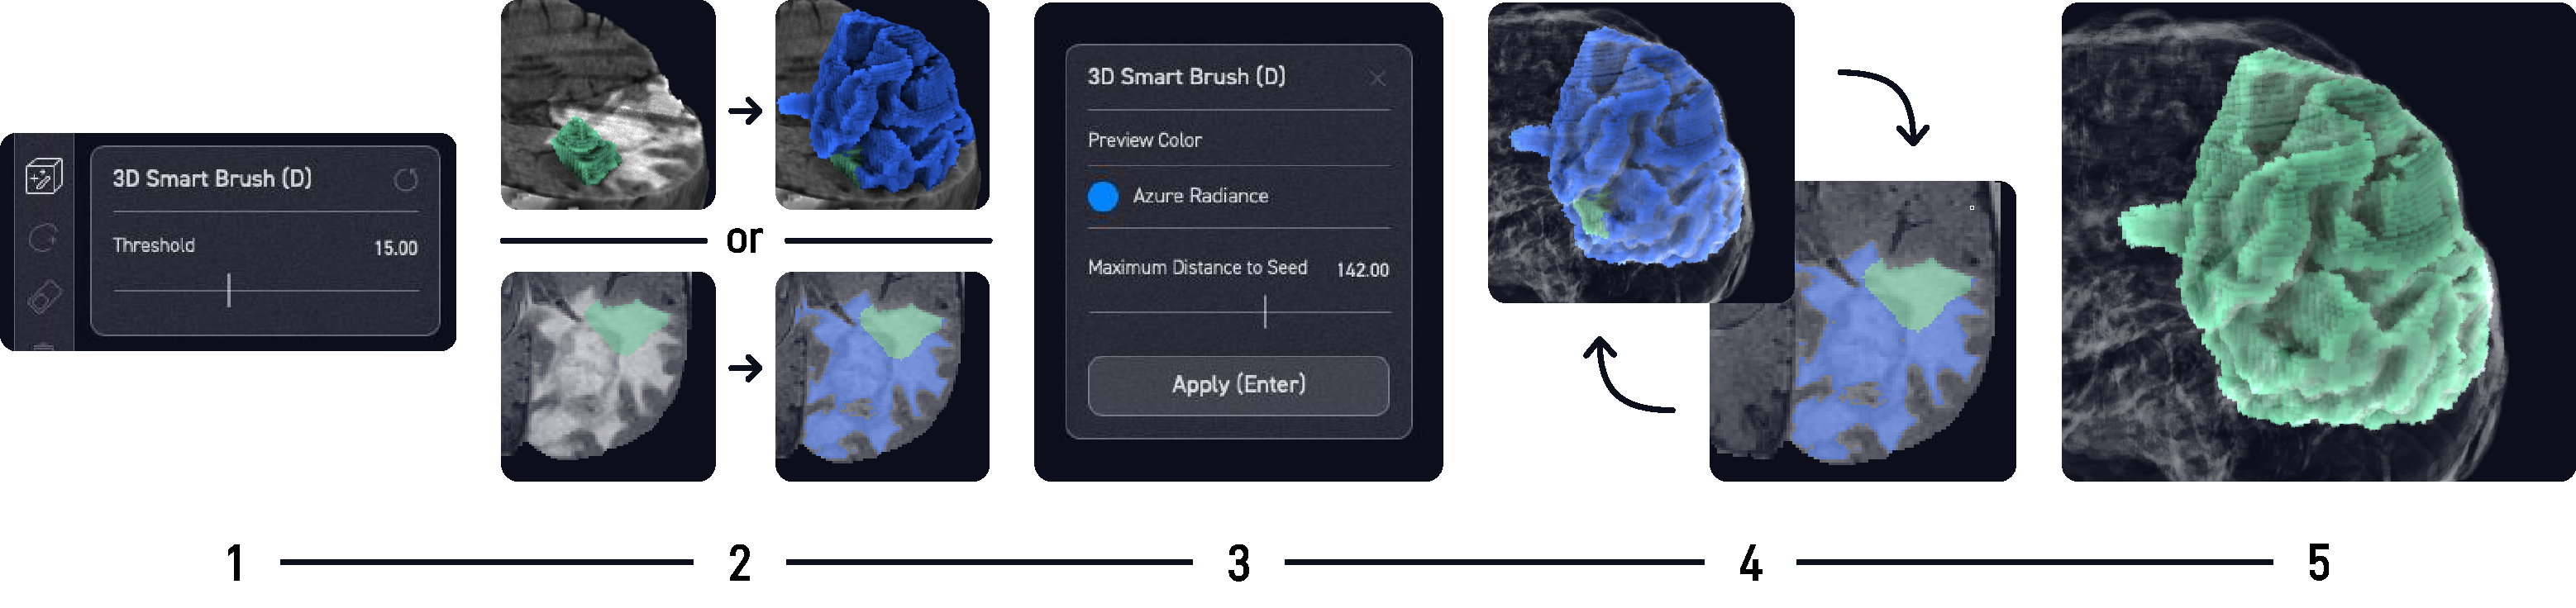
\includegraphics[width=\textwidth]{figures/workflow.pdf}
  \caption{Workflow for using 3D region growing to segment a brain tumor in an MRI.
1: Select desired threshold.
2: Select seed in 2D or 3D. System performs region growing. Region growing preview is rendered in both 2D and 3D.
3: Panel with tuning settings is shown.
4: Use slider from panel to adjust region growing distance. View in 2D and 3D to find errors.
5: Confirm the segmentation.}
  \label{fig:workflow}
\end{figure*}

\section{Volumetric Segmentation}
\label{3d_seg}
Segmenting a volumetric structure such as brain tumors slice by slice takes a long time. Computer-assisted annotation tools that perform region growing based on a user-selected seed can accelerate this workflow without additional data requirements~\cite{chen2017clipping,top2011al}.
However, without any knowledge about the structure the user intends to segment, region growing algorithms tend to easily over-grow the expected area by a large amount. This is why region growing tools are often limited to segment one slice at a time, enabling users to judge the correctness of the grown region accurately.

To enable confident atomic segmentation of a whole 3D volume, we thus use a combination of the standard two-dimensional slice-based rendering and three-dimensional direct volume rendering. This helps users to recognize large over-grown areas rapidly.

Additionally, we do not force the user to discard the whole grown region, should any error occur. Instead, we provide them with a preview that they can interactively tune to scale back how far the region is allowed to grow from the seed. This way, it is possible to limit the grown region in a way that it cannot \enquote{escape} the intended bounds while still keeping as much as possible of the desired segmentation. Whether or not the grown region escapes the user-intended bounds can be judged in the context of a visualization of prominent edges in the MRI scan (\cref{fig:teaser}, right).

\paragraph{Mathematical Model}
As mentioned in \cref{introduction}, we use a very simple mathematical model for region growing in order to avoid additional bias when using the result for training machine learning models.
Let $I_\textrm{seed}$ be the MRI intensity of the selected seed voxel, $I_\textrm{self}$ the MRI intensity of a voxel that could become part of the region, $I_\textrm{neighbor}$ the MRI intensity of a neighboring voxel, and $t$ the region growing threshold.
Then, the voxel becomes part of the region if the neighboring voxel is part of the region, and $|I_\textrm{self} - I_\textrm{neighbor}| < t$, and $|I_\textrm{self} - I_\textrm{seed}| < 1.5 t$.
This has to be tested for all six neighboring voxels.
Using $I_\textrm{seed}$ ensures that the region cannot grow infinitely far away from the seed intensity in case there are smooth gradients in the MRI.

\paragraph{Workflow}
The specific workflow of our 3D region growing tool is shown in~\cref{fig:workflow}.
In the first step, the user sets the threshold used for region growing. 
This threshold controls the maximum difference between neighboring voxels' intensities that allows the region to grow.
In the second step, the user selects the seed region.
This can be done in both the 2D and the 3D views.
In the 2D view, the user can scroll through the slices of the MRI and select the seed voxel using the mouse cursor.
In the 3D view, the user can click anywhere in the rendered image and the seed will be set at the first high-opacity intersection of their click with the volume.
This works especially well when using the cone transfer function (see \cref{fig:workflow}, step 2) as it allows the user to set the seed somewhere in the middle of the tumor and not only on the outside of the brain.
After that, the region growing is executed.
The grown region is shown as a preview in a distinct color to differentiate it from any pre-existing segmentation parts. 
Furthermore, a tuning UI panel is automatically opened, giving the user access to a slider that controls the maximum distance the region may grow from the seed. 
\Cref{fig:regiongrowing} shows the effect of manipulating the slider from within the 3D view.
In the fourth step, the user can switch between the 2D and 3D view while manipulating the slider to ensure there are no large errors where the region over-grew the desired part of the volume. 
As guidance, different transfer functions (detailed in \cref{dvr}) can be used, e.g., one that shows prominent edges in the underlying MRI, which can be useful to judge whether the grown region has escaped the intended section of the volume or not. 
Finally, in the fifth step, the user applies the previewed region to merge it into the segmentation volume.

\paragraph{Integration} 
Our 3D region growing workflow is integrated into a 2D segmentation web application called \emph{VISIAN}%
    \footnote{\emph{VISIAN} is a web-based image segmentation suite with a focus on machine learning in the medical domain. Please refer to \href{https://visian.org}{https://visian.org} for more information.}.
This means that smaller clean-up and voxel-level corrections can be performed in 2D after the 3D region growing has been completed. For this, \emph{VISIAN} includes multiple tools such as a simple pixel brush and eraser, 2D region growing, and outlining to add and remove voxels to and from the segmentation. Additionally, interactive dilation and erosion filters can be used to fill small holes or remove unwanted noise in the segmentation.
Due to this integration, a hybrid 2D and 3D workflow for segmentation becomes feasible.

\begin{figure*}[t]
    \begin{tikzpicture}[%
        every node/.append style={shape=rectangle, rounded corners=2mm}, %
        spy using outlines={white, rectangle, magnification=2.5, size=56, connect spies, every spy on node/.append style={line width=1.0pt}}, %
        inner sep=0pt, outer sep=0pt]
        \node[anchor=west, clip](scans) at (0,0) {%
            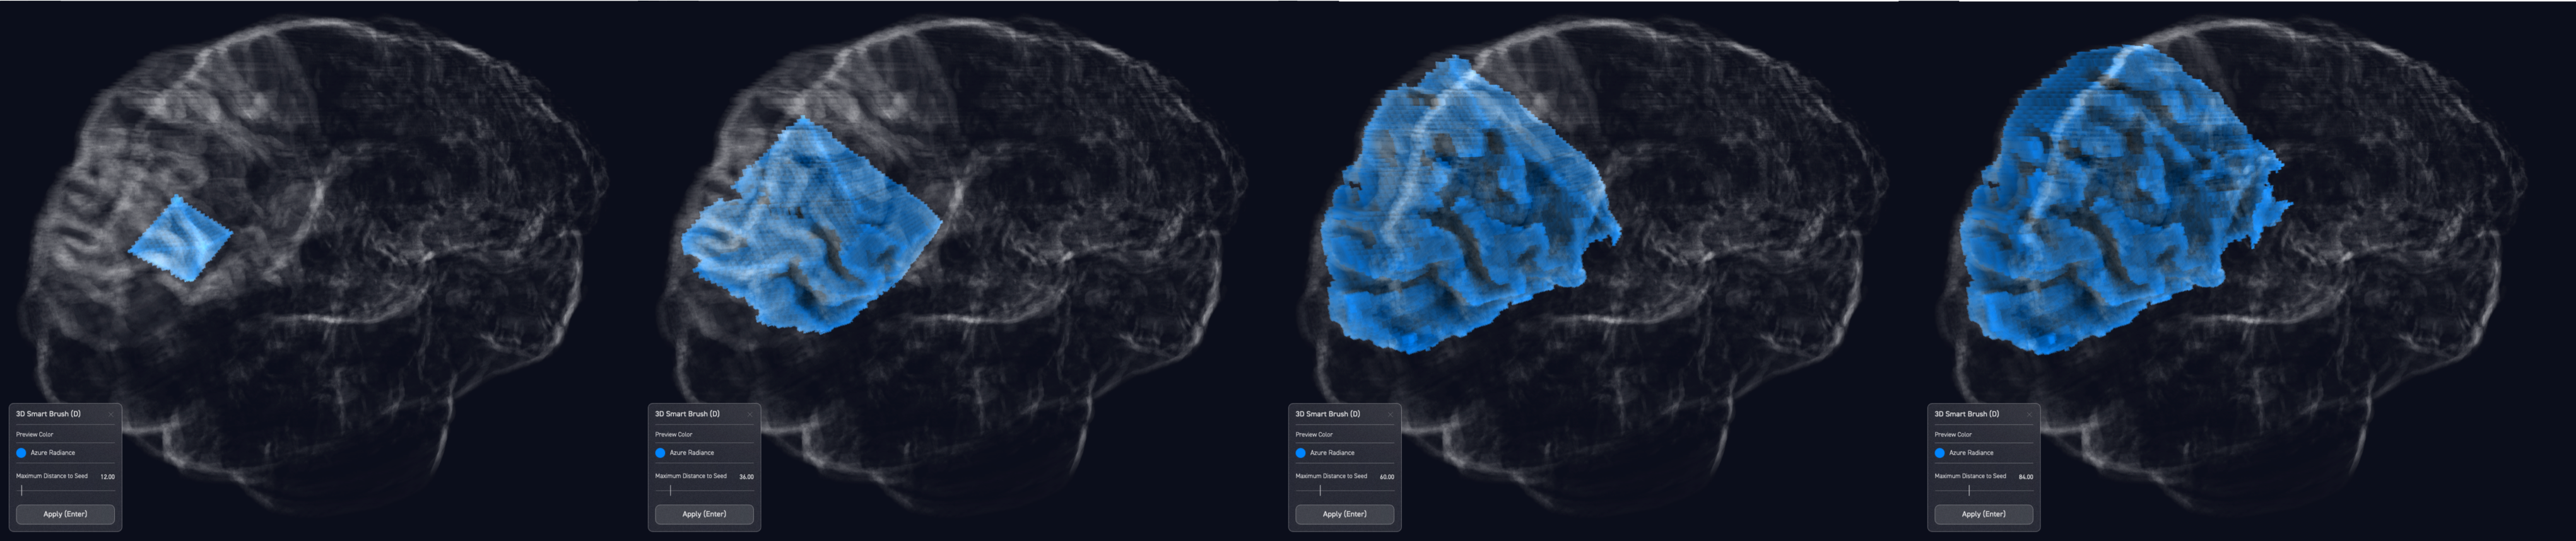
\includegraphics[width=1.0\linewidth, trim=0 0 0 0, clip]{figures/regiongrowing}};
        \spy on ($(scans.center)+(-4.03, -1.32)$) in node at ($(-5.8, -0.5)+(scans.center)$);
    \end{tikzpicture}
    \caption{3D region growing of a brain tumor segmentation restricted to different numbers of region growing steps; 12, 36, 60, 84 f.l.t.r. respectively. Note that the segmentation is contained in the visible tumor edges.}
    \label{fig:regiongrowing}
\end{figure*}

\section{Direct Volume Rendering}
\label{dvr}
In this section, we briefly describe the \emph{transfer functions} used in our volume rendering, discuss aspects on \emph{medical correctness} of the rendering itself, and highlight our \emph{progressive rendering} approach.

\paragraph{Transfer Functions}
To display MRIs and segmentation volumes in 3D, we provide multidimensional transfer functions, namely  $H_\textrm{dense}$, $H_\textrm{clip}$, $H_\textrm{edge}$, and $H_\textrm{user}$, used for ray tracing (more specifically, ray marching).
Transfer function $H_\textrm{dense}$ maps the MRI intensities to opacity and grayscale of the volume (\cref{fig:teaser}, left). 
The displayed intensity values can be filtered from top and bottom, and the segmentation volumes can be used to mask them.
Transfer function $H_\textrm{clip}$ uses selective spatial clipping to enable \emph{focus+context} visualization. 
The focus is put on the segmentation volumes while the MRI scans are used for context and spatially clipped by a cone (\cref{fig:teaser}, middle). 
The cone can follow the virtual camera or be fixed in place. 
A similar approach for selective spatial clipping, presented by~\citeauthor{diaz2012_clipping}, used a clipping plane instead of a cone (which can be seen as a special case of a 180\si{\degree} cone).
$H_\textrm{edge}$ semi-transparently displays pronounced edges in the MRI scans around the segmentations to give spatial context information while barely occluding the focus volumes (\cref{fig:teaser}, right).
The edges are detected based on gradient magnitude~\cite{kniss2002multi_tfs} and can be filtered from top and bottom.
To allow for custom mapping of MRI intensity values to colors and opacities, a fourth transfer function, $H_\textrm{user}$, can be specified by custom, single-pixel-height images uploaded by the user.

\paragraph{Medical Correctness} 
While color, opacity, and shading within our 3D visualization collectively provide an expressive visual representation of the data, they also influence the perception of the data and might cause misrepresentation of the real anatomy~\cite{pommert2002correctness}. 
Therefore, we give users additional access to the raw MRI data by means of a 3D clipping plane that can be placed and oriented freely within the MRI volume (\cref{fig:plane}). 
If the plane is axis-aligned, the image displayed on the plane shows a typical MRI slice with square (or rectangular for non-isotropic scans) voxel shapes (\cref{fig:plane}, left).
Regardless of the plane orientation, however, nearest neighbor filtering is favored over linear interpolation to display only accurate and factual intensity values (\cref{fig:plane}, right).

\begin{figure}[b]
    \begin{tikzpicture}[%
        every node/.append style={shape=rectangle, rounded corners=2mm}, %
        spy using outlines={white, rectangle, magnification=3.0, size=56, connect spies, every spy on node/.append style={line width=1.0pt}}, %
        inner sep=0pt, outer sep=0pt]
        \node[anchor=west, clip](scans) at (0,0) {%
            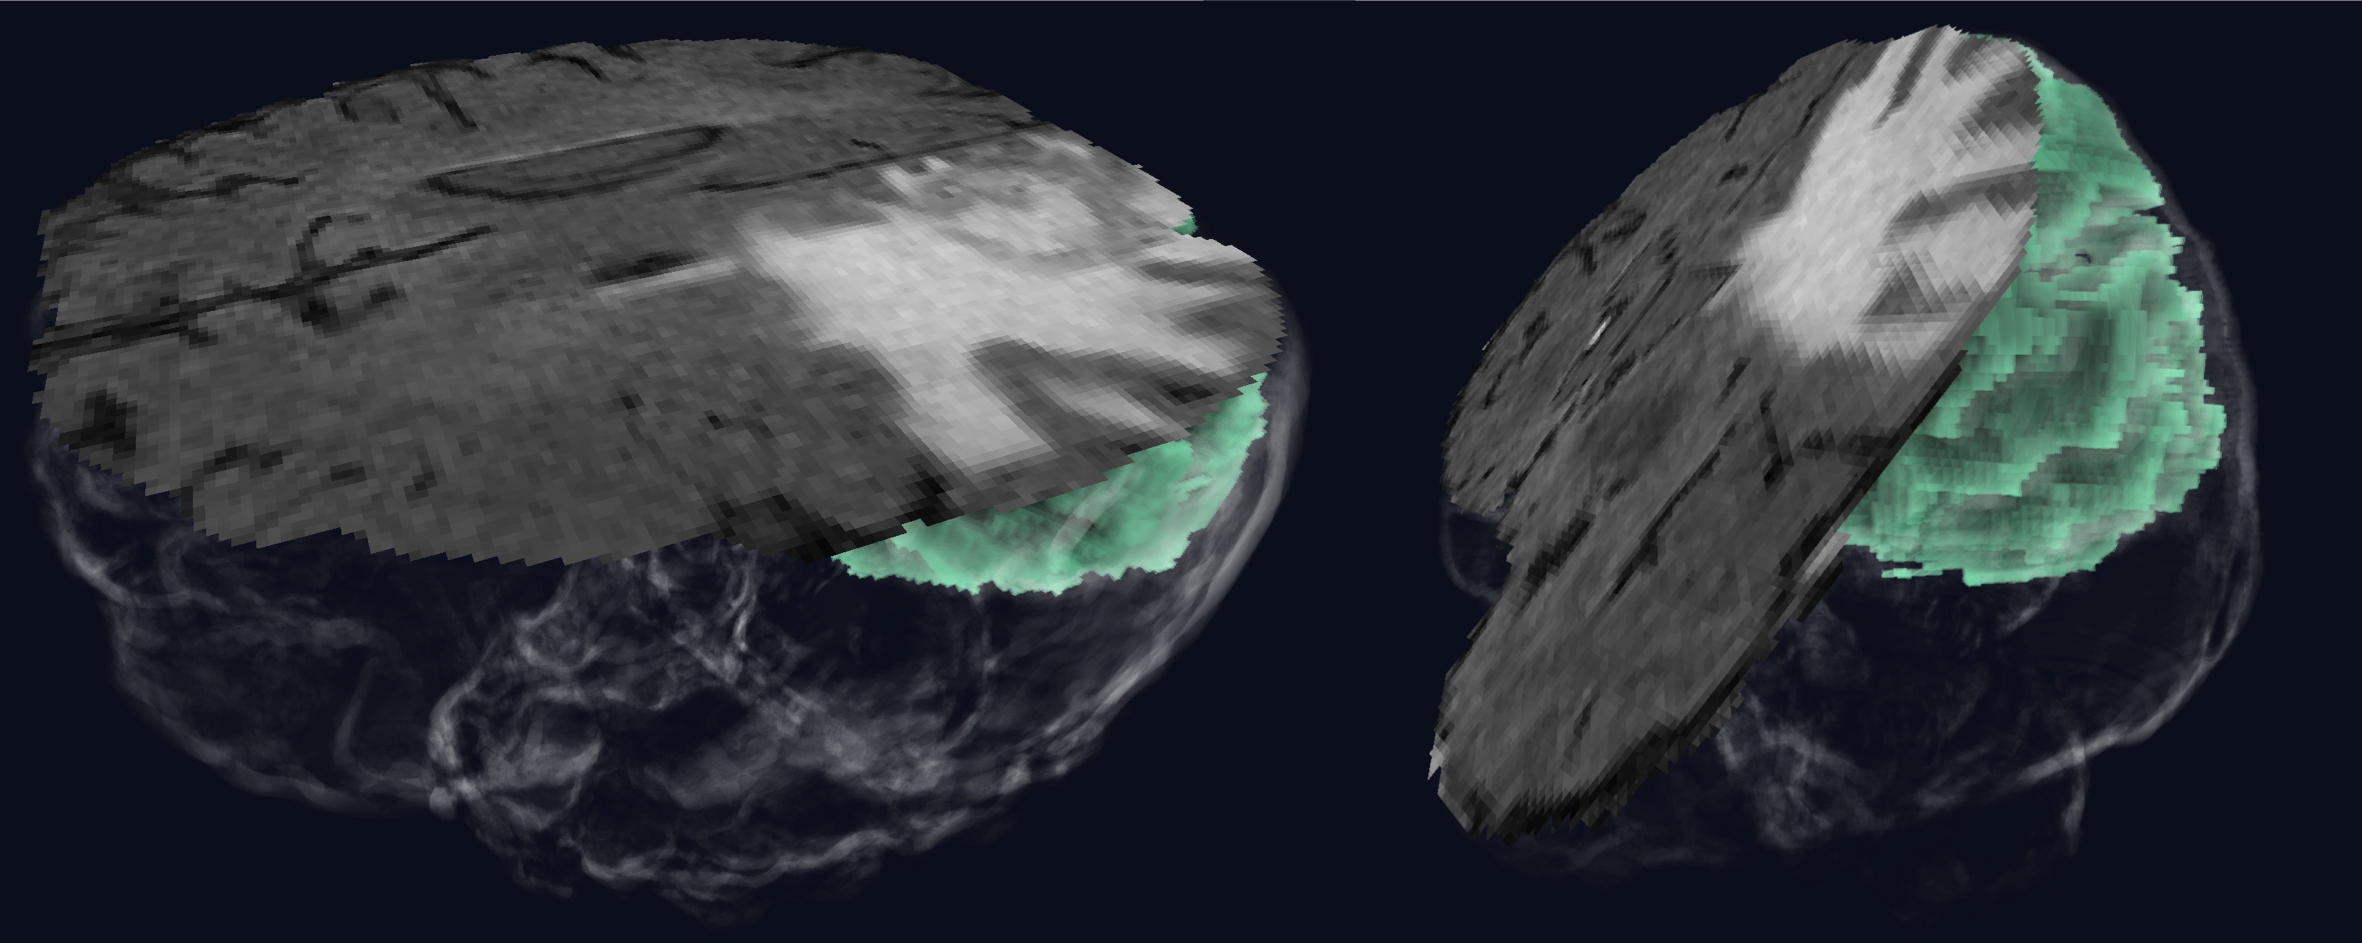
\includegraphics[width=1.0\linewidth, trim=0 0 0 0, clip]{figures/plane}};
        \spy on ($(scans.center)+(+0.0, +0.25)$) in node at ($(-3.0, +0.45)+(scans.center)$);
    \end{tikzpicture}
    \caption{Raw MRI data is shown on a clipping plane through the volume. Axis-aligned (left) and freely oriented (right).}
    \label{fig:plane}
\end{figure}

\paragraph{Progressive Rendering} 
To achieve interactive frame rates even on low-performance devices, we use progressive rendering for resolution and shading quality. 
In particular, when the user moves the virtual camera, the resolution is decreased immediately and progressively increased once the movement has stopped. 
This allows for both a smooth frame rate during interaction and full-quality images once the desired perspective is found. 
For shading, we use progressive local ambient occlusion (LAO), which determines the occlusion (darkening) of a particular voxel by sampling short rays in multiple directions~\cite{hernell2010LAO} over multiple frames.
For every frame, only a few rays are used, and the results are accumulated over time.
Thereby, the shading quality continuously increases.
This shading remains valid regardless of camera movement.
It is invalidated only when the volume display configuration changes, e.g., through clipping or transfer function changes.

\section{Implementation}
\emph{VISIAN} is built in TypeScript using React with MobX for state management and runs exclusively on the client.
For graphics, we use Three.js as a wrapper around WebGL. 
Since we built \emph{VISIAN} with tablet and especially iPad users in mind to enable pen input for segmentation, we decided to use WebGL 1. 
This means that we cannot use 3D textures. 
Instead, we use texture atlases that contain all slices of a scan next to each other. 
This has positive and negative effects. 
It makes it easy, e.g., to generate textures that contain gradient information used for detecting edges. 
We can simply render the whole atlas at once with a corresponding fragment shader and do not have to render slice by slice.
However, it also means that we cannot use the hardware's trilinear interpolation. 
Instead, we have to use the hardware's bilinear interpolation and perform a third mix manually in a shader.
With the expected upcoming ratification of WebGPU, a switch from WebGL to WebGPU seems very promising since it might resolve the current workarounds and limitations while improving the overall performance of our application.

In the following, implementation details on \emph{ray tracing}, \emph{GPU-based 3D region growing}, and \emph{progressive rendering} are provided.

\begin{figure}[b]
    \begin{tikzpicture}[%
        every node/.append style={shape=rectangle, rounded corners=2mm}, %
        spy using outlines={white, rectangle, magnification=3.0, size=56, connect spies, every spy on node/.append style={line width=1.0pt}}, %
        inner sep=0pt, outer sep=0pt]
        \node[anchor=west, clip](scans) at (0,0) {%
            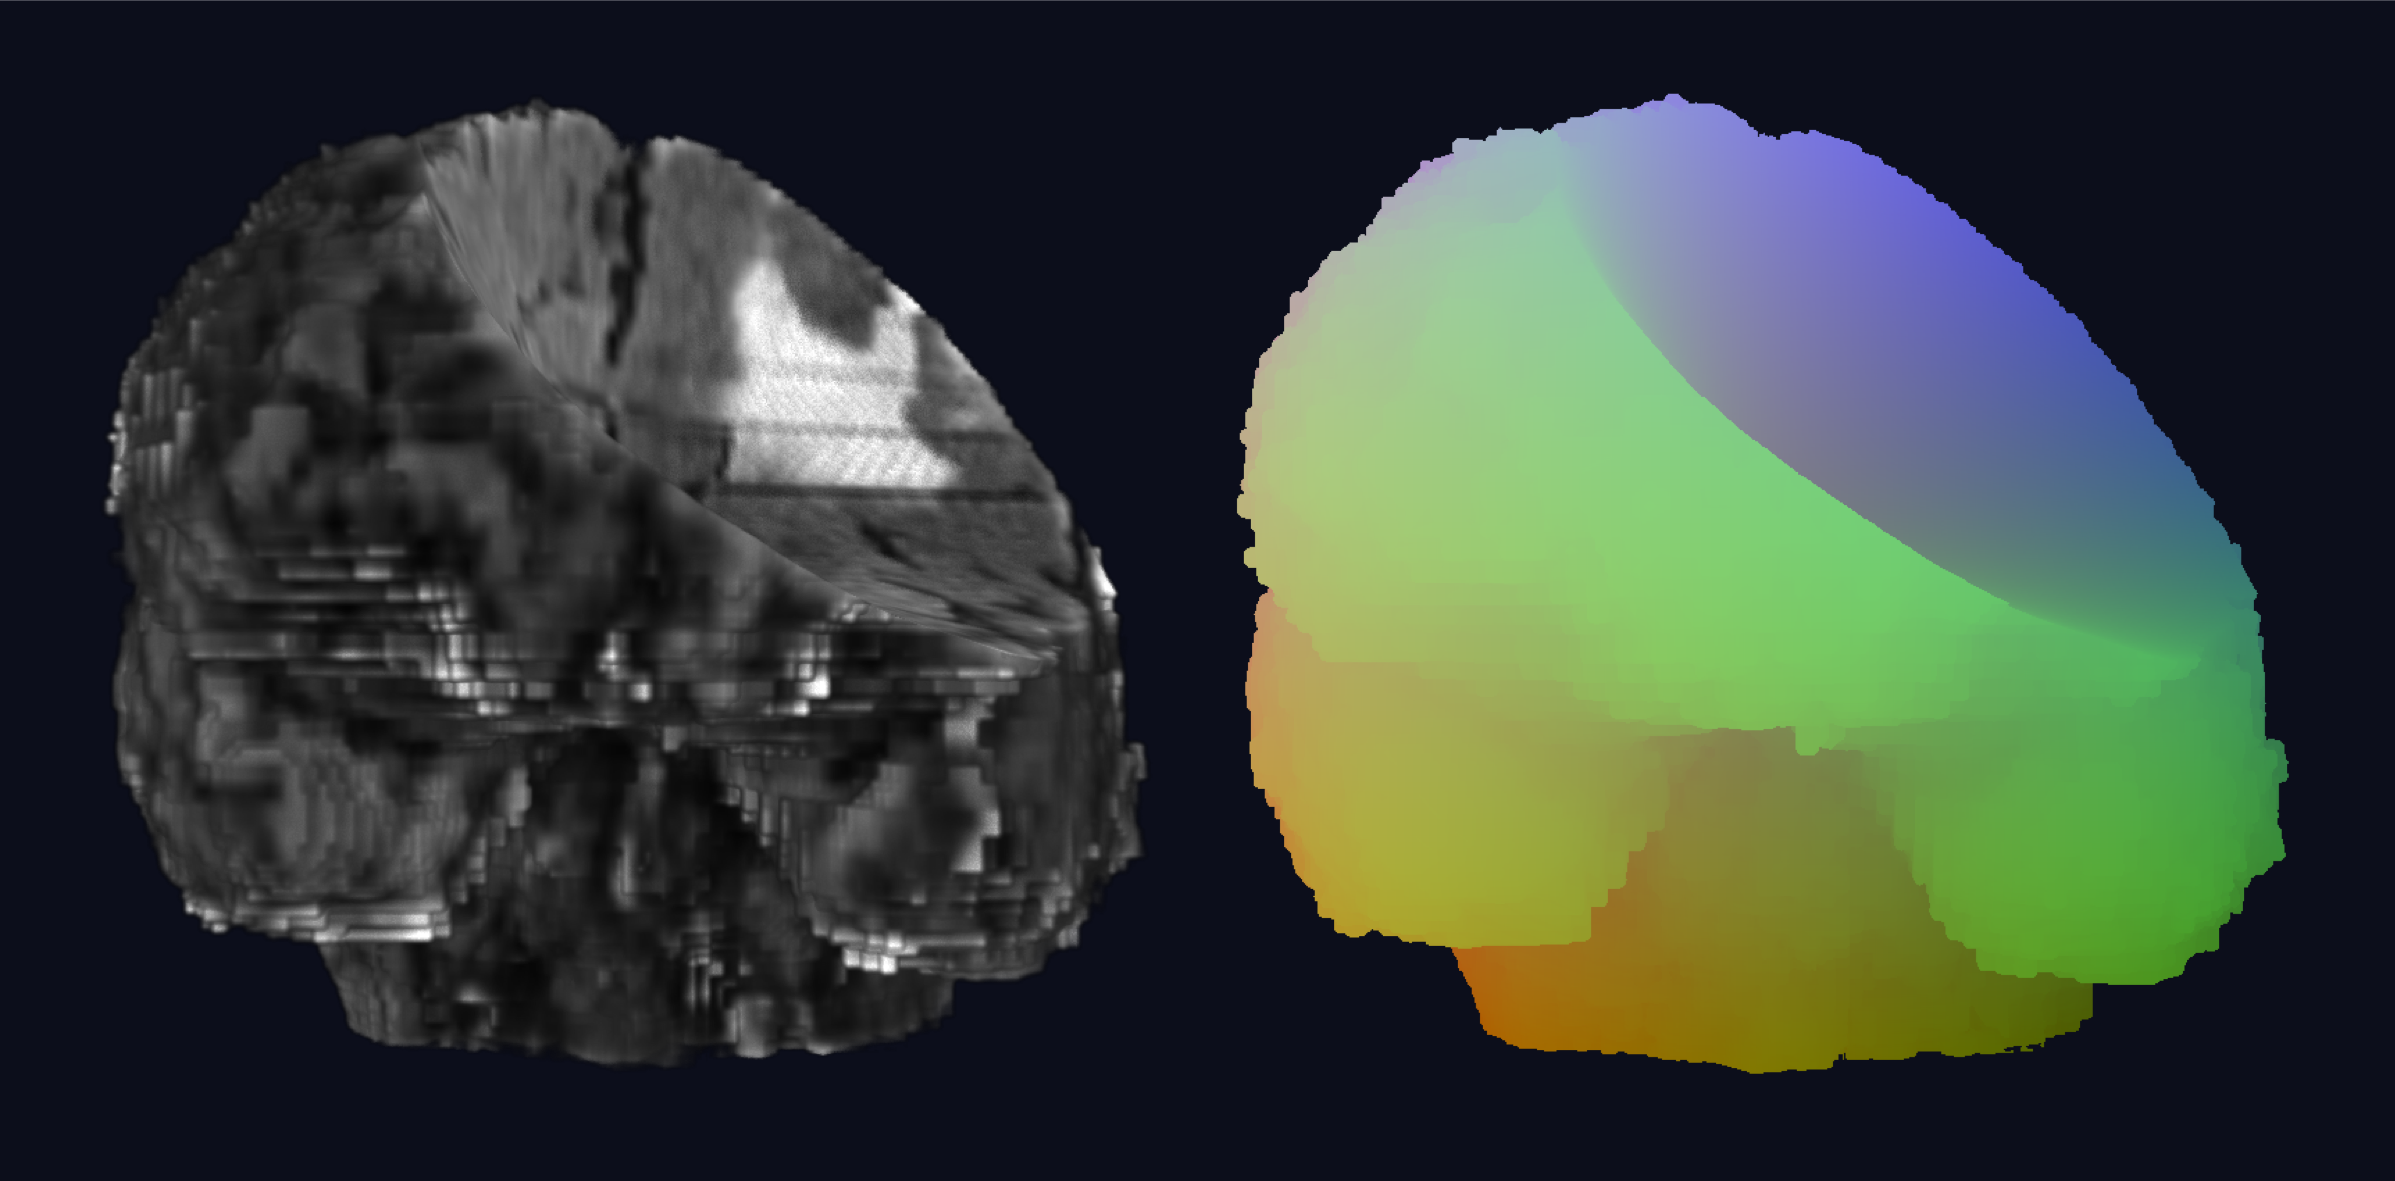
\includegraphics[width=1.0\linewidth, trim=0 0 0 0, clip]{figures/picking}};
    \end{tikzpicture}
    \caption{Brain MRI with a tumor rendered using the $H_\textrm{clip}$ transfer function. Normal volume shader showing the tumor as a potential region growing seed location in white (left) and volumetric picking shader (right).}
    \label{fig:picking}
\end{figure}

\begin{figure*}[t]
  \centering
  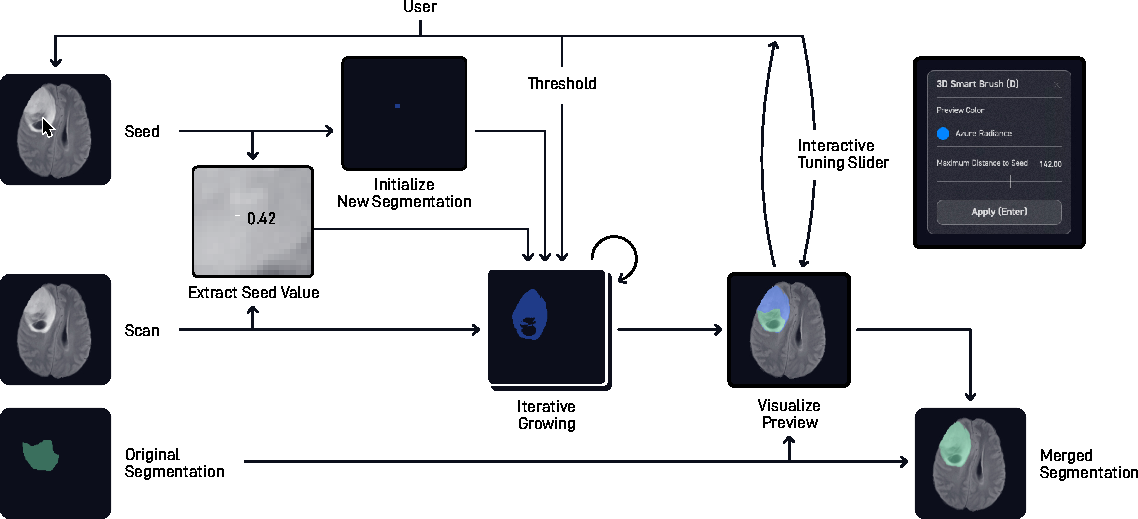
\includegraphics[width=\textwidth]{figures/data_flow.pdf}
  \caption{Data flow of the region growing process.
  The process is initiated by the user when selecting a seed position.
  From this, an initial segmentation containing only the selected voxel is created, and the seed value is extracted from the underlying scan.
  In the iterative growing phase, this initial segmentation then grows iteratively based on the extracted seed value, the underlying scan, and the user-defined threshold.
  The grown segmentation is then visualized as a preview together with the original segmentation and the user can interactively tune how far the region may grow from the seed using the tuning slider.
  Finally, the tuned segmentation is added to the original one to form the merged segmentation.}
  \label{fig:data_flow}
\end{figure*}

\paragraph{Ray Tracing}
For the initial rays, the back faces of the volume's bounding box are rasterized and used for subsequent, custom ray marching through the MRI volume (utilizing fragment shaders for computation).
This simplifies further composition of other auxiliary meshes like clipping plane (\cref{fig:plane}) or VR controllers rendered directly using Three.js.
To render multiple MRI scans and segmentations simultaneously, we use a stack of layers. 
During ray marching, we blend the colors and opacities of all layers at every sample point along the rays according to the stack's layer sequence. 
This allows the user to rearrange layers such that more important segmentations show up more dominantly when overlapping with other segmentations.
Furthermore, this unifies the 2D and 3D experience as the layers are blended in the same way for the 2D view.

To push all layers onto the GPU, we use a columnar uniform layout in the fragment shader. 
However, since WebGL 1 only allows constant array lengths for uniforms, we apply custom regex macros to compose the desired shader code and adjust it to the required number of layers.

\begin{figure*}[t]
  \centering
  \begin{tikzpicture}[%
        every node/.append style={shape=rectangle, rounded corners=2mm}, %
        spy using outlines={white, rectangle, magnification=2.0, size=64, connect spies, every spy on node/.append style={line width=1.0pt}}, %
        inner sep=0pt, outer sep=0pt]
        \node[anchor=west, clip](scans) at (0,0) {%
            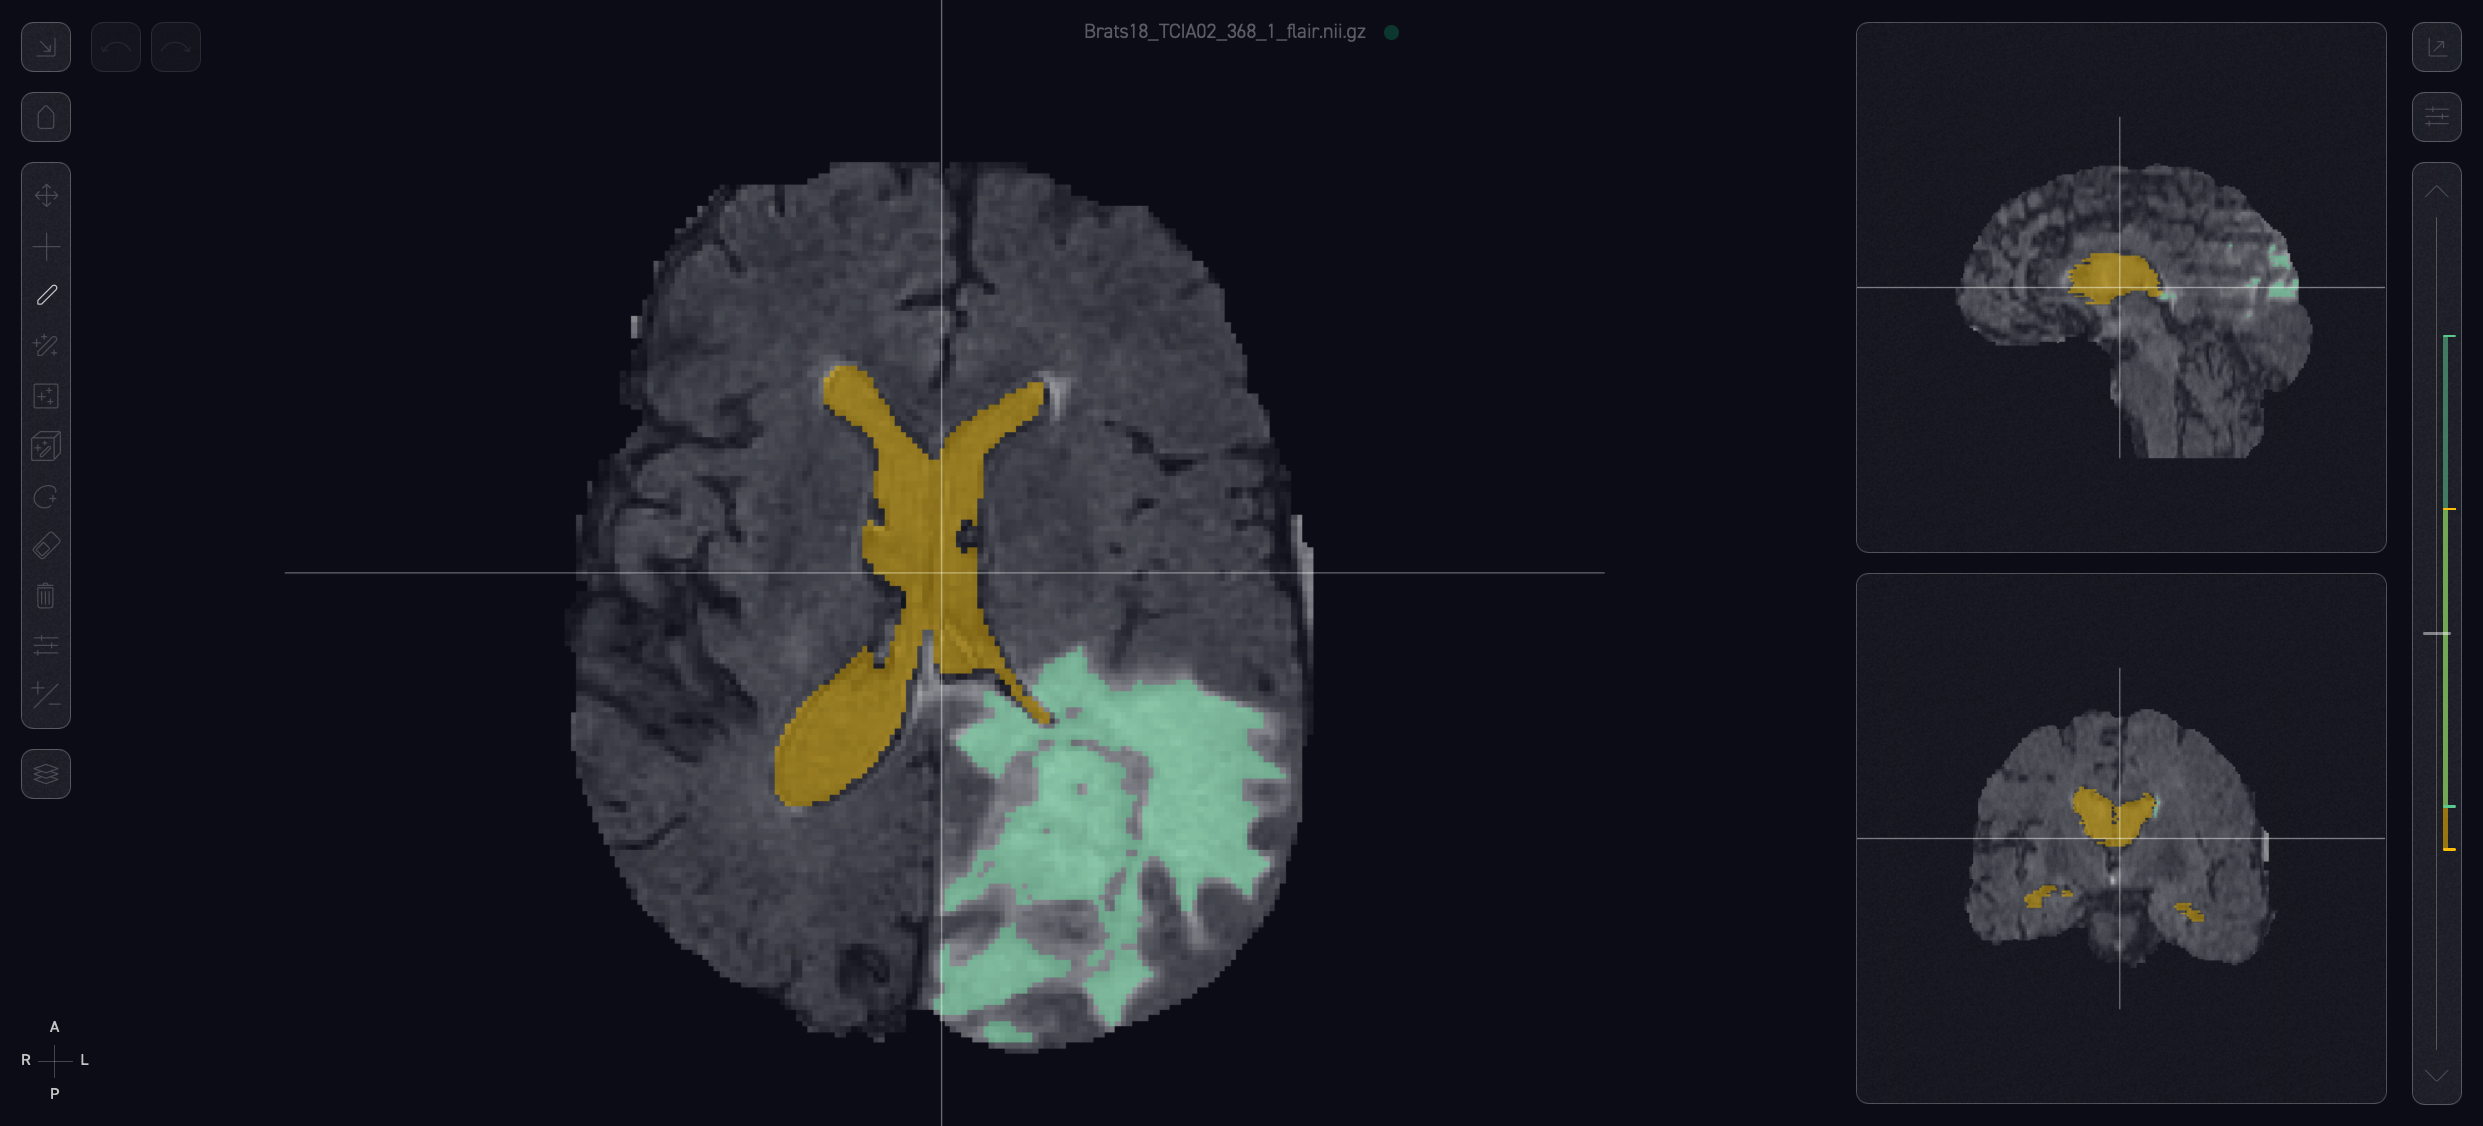
\includegraphics[width=1.0\linewidth, trim=0 0 0 0, clip]{figures/visian2d}};
    \end{tikzpicture}
  \caption{\emph{VISIAN's} 2D interface showing a brain MRI with segmentations of a tumor (green) and the ventricles (yellow).}
  \label{fig:visian2d}
\end{figure*}

\paragraph{3D Seed Selection}
To place a seed for region growing in the 3D view the user clicks onto the rendered image.
To convert the 2D click position into the corresponding 3D position in the volume, volumetric GPU picking is used, rendering the volume again off screen with a modified shader.

This modified shader does the same front-to-back ray marching and color accumulation as the normal volume shader.
However, when a small opacity threshold (in our case $0.01$) is reached, the ray marching loop is terminated and the current normalized volume coordinates from the ray marching process are rendered into the r, g and b channels of the output buffer.
To indicate that the ray marching hit a target, $1.0$ is rendered into the alpha channel.
See \cref{fig:picking} for a side-by-side comparison of a brain MRI rendered with the $H_\textrm{clip}$ transfer function and its corresponding volumetric GPU picking shader.
If no high opacity is reached, i.e., the user clicked onto the background, this is indicated by a $0.0$ in the alpha channel.
The same kind of shader is used for the clipping plane (\cref{fig:plane}) during the picking process. 
However, as this is a normal, rasterized geometry, no ray marching is needed here. 
The rendered normalized volume coordinates are then converted to the corresponding voxel information, which is then used as the seed for region growing.

\lstinputlisting[%
    float = b, %
    language = glsl, %
    label = lst:regiongrowing, %
    caption = {%
        GLSL shader that decides for each voxel whether the region should grow onto it from one of its six neighbors.}%
    ]{region-growing.glsl}

\paragraph{GPU-based 3D Region Growing}
The data flow involved in the tunable 3D region growing process is depicted in \cref{fig:data_flow}.

The region growing itself iteratively runs on the GPU. 
We use two frame buffers and render back and forth between them by using them as alternating input and output.
In each step, the region can grow one step. 
As we are using a texture atlas instead of a 3D texture, we render the whole atlas at once.
For this, we use a screen-aligned quad and a fragment shader to compute the region growing for each voxel (\cref{lst:regiongrowing}). The same procedure is also used to enable multi-step dilation/erosion for segmentation clean up.

To allow for interactive adjustment of the maximum region growing distance (\cref{fig:regiongrowing}), we encode the step in which a voxel first became part of the region using 8 bit in one of the texture's channels. 
Based on this value, we filter the preview using the user-controlled slider value. To render the preview, an additional annotation layer is placed on top of the layer stack.
When applying the previewed segmentation to the existing one, we use the filter and render the voxels additively into the segmentation's texture atlas.
Encoding the step number in 8 bits allows us to grow the region by 254 steps ($0$ is reserved for voxels not part of the region, and $255$ is the seed). 
More channels could be used to encode more steps.
However, this would also linearly increase the time it takes to perform the region growing, as would increasing the size of the scan.
For common scan resolutions used in brain tumor segmentation, 254 steps are typically sufficient to segment whole tumors.

The region growing itself operates on the raw MRI intensities. 
It uses the selected seed's and the six neighboring voxels' intensities for thresholding when growing the region to adjacent voxels (see \cref{3d_seg} for the mathematical model and \cref{lst:regiongrowing} for an implementation in a GLSL fragment shader).
Whenever the user changes the region growing distance, voxels are added or removed from the preview (\cref{fig:regiongrowing}) without recomputation. 
However, this means that the LAO for all voxels needs to be recomputed. 
Since this is a computationally intensive operation, we momentarily turn off shading updates while the user changes the distance.

\paragraph{Progressive Rendering}
For progressive rendering, tiled rendering is used.
In particular, rendering a higher resolution of the image is not done all at once.
Instead, smaller tiles are rendered and stitched together at the desired resolution.
This allows aborting rendering of higher resolutions quickly, e.g., when the user moves the virtual camera again. 
The LAO texture atlas is rendered tile-based as well.
Here, the results of the previous rendering step are reused and accumulated.
This way, we can start with only a few LAO rays, e.g., eight, and progressively produce a full resolution image with this first shading iteration. 
Then, another batch of LAO rays is rendered and accumulated.
With the resulting LAO texture atlas, a full resolution image is rendered off-screen and swapped with the \enquote{low-cost} screen image once it is ready. 
This process is repeated until a target number of LAO rays is reached (32 by default).

\section{Results}
\label{results}

Our approach achieves an end-to-end 3D segmentation workflow that extends the 2D user interface of the image annotation system \emph{VISIAN} as seen in \cref{fig:visian2d}.

\paragraph{Performance}
We tested our implementation on a local development deployment of \emph{VISIAN} running in Chrome 92.0.4515.107 (64-bit) on a workstation equipped with an i7-7700K running at 4.50 GHz, 32 GB of 3000 MHz DDR4 RAM, an Nvidia GeForce RTX 2070 SUPER, and a 4K display.

\Cref{tab:computationtimes} shows the computation times for all 254 region growing steps on a scan from the BraTS 2018 dataset~\cite{brats1,brats2,brats3} of resolution $240\times240\times155$, resulting in a texture atlas resolution of $3120\times2880$. As evident, the first run completed in just below $40 ms$ with precompiled shaders. In our tests, it took $10 - 20 ms$ longer if the required shaders had not been precompiled. Due to caching effects, the following consecutive region growing runs on the same scan completed in, on average, $5 ms$.

All proposed transfer functions produced stable 60 fps video output using our progressive rendering on the above hardware.
Without our progressive resolution, the frame rate, depending on the zoom level, occasionally dropped to as low as 20 fps.

\begin{figure}[t]
    \begin{tikzpicture}[%
        every node/.append style={shape=rectangle, rounded corners=2mm}, %
        spy using outlines={white, rectangle, magnification=3.0, size=56, connect spies, every spy on node/.append style={line width=1.0pt}}, %
        inner sep=0pt, outer sep=0pt]
        \node[anchor=west, clip](scans) at (0,0) {%
            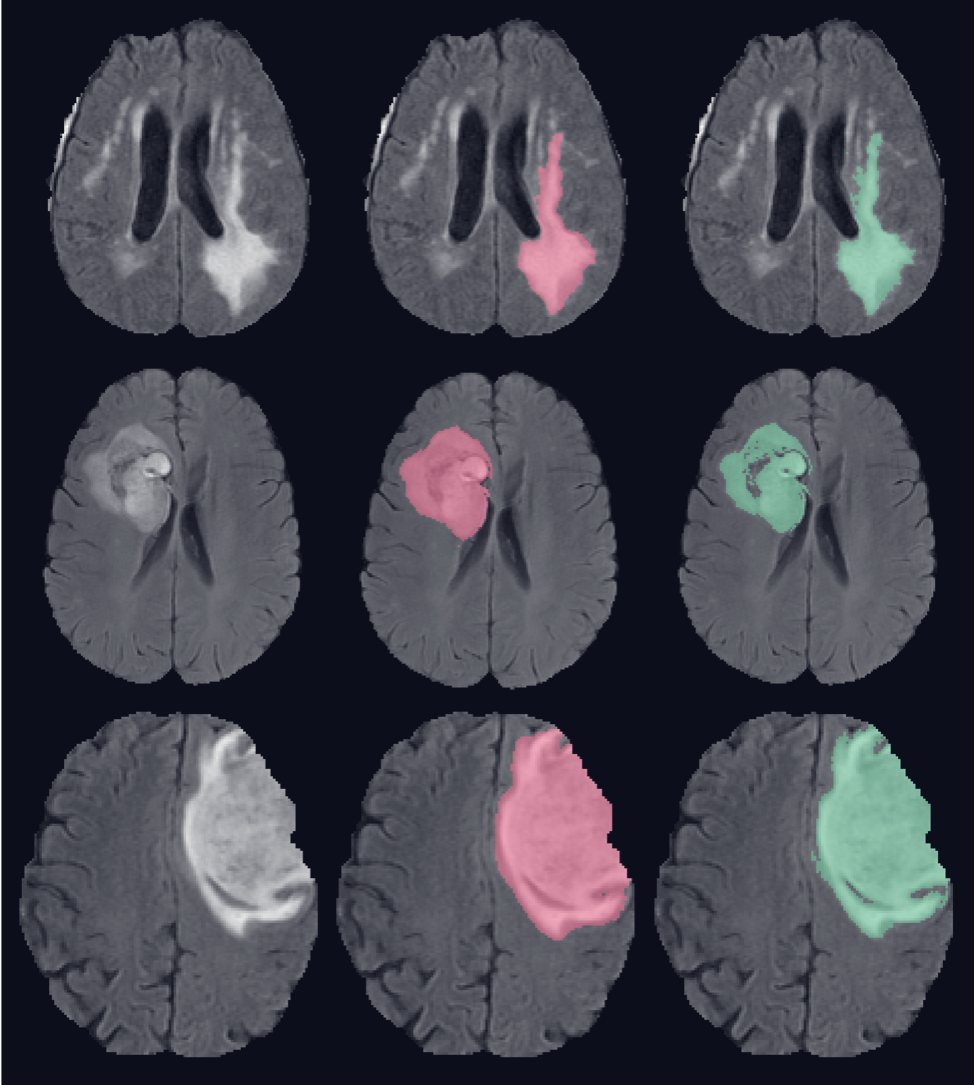
\includegraphics[width=1.0\linewidth, trim=0 0 0 0, clip]{figures/ground-truth}};
    \end{tikzpicture}
    \caption{Comparison of expert ground truth annotations (red, middle) and amateur annotations using the volumetric region growing tool (green, right) on the raw scans (left). Note the small holes in the region growing annotations (green, right) in the 2nd and 3rd rows. These occur because parts of the tumor core appear darker in FLAIR MRI which stops the region growing algorithm. Using the dilate/erode post-processing can fill such holes.}
    \label{fig:ground-truth}
\end{figure}

\paragraph{Segmentation Quality}
A first qualitative evaluation of our region growing approach on FLAIR-modality BraTS scans showed that it can produce glioma segmentations that require very little tweaking to achieve accurate outer boundaries.
\Cref{fig:ground-truth} shows a comparison of three expert-annotated ground truth segmentations (red, middle) and amateur segmentations using our volumetric region growing workflow (green, right) on the raw scans (left). All three scans and ground truth segmentations come from the BraTS 2018 dataset.
The ground truth segmentations were created by multiple experts using multiple scan modalities (see~\cite{brats2} for more details), while the region growing segmentations were created by an amateur using only the volumetric region growing workflow described in \cref{fig:workflow} and only the shown FLAIR modality.

However, as the core of gliomas can yield fundamentally different image intensities from its surroundings, the generated segmentations often contained a hole in their center (see \cref{fig:ground-truth}, rows 2 and 3).
Placing a second seed or using the dilation/erosion post-processing described in \cref{3d_seg} could typically fill these holes.

Especially small holes in the generated segmentation that can often be fully occluded proved hard to find in the volumetric 3D view. We deduce that our current transfer functions can speed up the segmentation proofing process, but they cannot yet replace the 2D view for the task of voxel-exact proofing. However, they were particularly helpful when tuning the maximum number of region growing steps as changes to it became immediately visible on the outside of the generated segmentation.

\begin{table}[t]
    \centering
    \small
    \renewcommand{\arraystretch}{1.2}
    \begin{tabularx}{\linewidth}{X|rrrrr}
        \footnotesize\textbf{Run Number} %
            & \#1 & \#2 & \#3 & \#4 & Mean of \#5--\#50 \\%
        \midrule %
        \footnotesize\textbf{Computation Time in \si{\ms}} %
            & $37.3$ & $26.8$ & $11.2$ & $6.6$ & $4.93\pm0.74$ \\
    \end{tabularx}
    \vspace*{2mm}
    \caption{Wall clock times for consecutive, user-initiated runs of all 254 region growing steps on a $240\times240\times155$ scan.}%
    \label{tab:computationtimes}
\end{table}

\section{Conclusion and Future Work}
Volumetric region growing can support quick segmentation of 3D structures in medical images such as brain tumors. 
By allowing the user to interactively scale how far a region can grow, unintended over-growing can be mitigated.
Another key to a successful 3D segmentation workflow is the tight integration of volumetric rendering with \emph{focus+context} visualizations into the segmentation process. 
This way, users can judge the volumes they are annotating in 3D and spot errors more quickly and easily.
Additionally, the 2D tools of a segmentation application such as \emph{VISIAN} can be used for effective clean up of grown regions.

Our progressive rendering approach is essential to
(1) maintain interactive frame rates on low-end devices while generating images of consistently high quality, %
(2) enable a responsive segmentation workflow, and %
(3) provide high resolution and high-quality shading to increase comprehension of volumetric structures.

In the future, \emph{VISIAN's} VR support could be used to set a seed region in 3D using controller input. 
Additionally, the presented 3D workflow could be extended by a \enquote{3D sculpting}-like brush tool that could add and remove voxels from the surface of a segmentation in 3D. While we do not find it likely that such a 3D correction workflow can fully replace voxel-level correction and proofing using the 2D view, we do believe it can save time when larger parts of a segmentation that span multiple slices have to be removed.
Finally, a comprehensive evaluation of our tool in real-world MRI segmentation tasks performed by clinicians is planned and important to steer subsequent research.

\begin{acks}
    We thank Maximilian Lindner for assistance with the graphics and \emph{VISIAN}'s user interface as well as Clara Uktar for help with \emph{VISIAN}'s development.
\end{acks}

\balance 
\bibliographystyle{ACM-Reference-Format}
\bibliography{references}

\end{document}
\endinput
